\section{Curve Tracing-Root finding}

The knowledge of maxima and minima can very well be used to figure out what the graph of a function looks like. It can be used to get a rough idea to guess the roots of a solution and even analytically unsolvable implicit equations. Okay, so let us take some examples:

\begin{enumerate}
    \item Draw the graph of $f(x)=x^2/\sqrt{x+1}$

    As we can see, the function is not defined for $x\leq -1$; the domain is $[1, \infty )$. Now, 
    $$\lim_{x \to -1^{-}} f(x) = \infty$$
    $$\lim_{x to \infty} f(x) \to x^{3/2}$$

    But how does it behave in between?
    If we differentiate the function, then we get:
    $$f'(x) = \frac{x(3x+4)}{(x+1)\sqrt{x+1}}$$

    This makes it clear that the extrema is achieved at x=0; if we consider the sign of the derivative on both sides of the extrema, we figure out that this extrema is a minima. And the value of the function at this minima is 0. \textbf{The the preliminary idea is that the function decreases from $\infty$ to 0, then increases, and for large values of x, it takes the form $x^{3/2}$}

    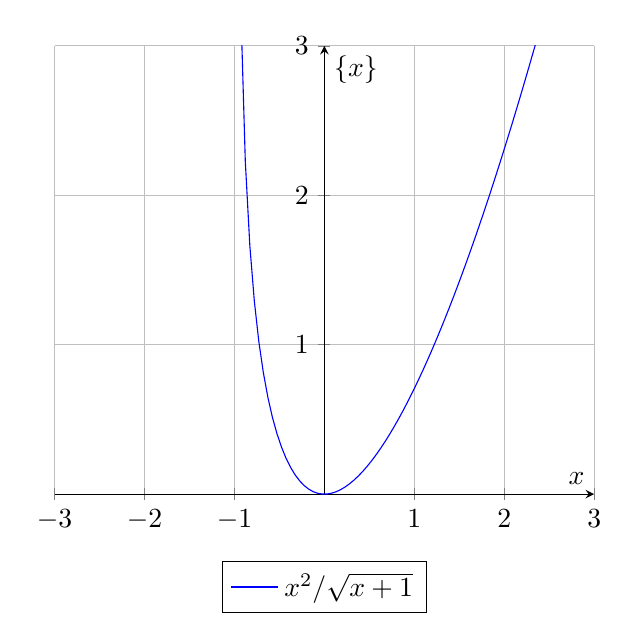
\begin{tikzpicture}
    \begin{axis}[
        xlabel={$x$},
        ylabel={$\{x\}$},
        xmin=-3, xmax=3,
        ymin=0, ymax=3,
        axis lines=middle,
        grid=both,
        legend style={at={(0.5,-0.15)},anchor=north}
    ]
    
    \addplot[blue, domain=-5:5, samples=200] {x^2/sqrt(x+1)};
    \legend{$x^2/\sqrt{x+1}$}
    
    \end{axis}
    \end{tikzpicture}

\item Let us draw the graph $xe^x$.

The domain is R. So, what happens at the extremal points?

At $x\to -\infty , f(x) \to 0$ and at $x \to \infty, f(x) \to \infty$

But what happens in between?

Let us differentiate the function and see:

$$f'(x)= (x+1)e^x$$

Thus, this function achieved a minimum at x=-1. And the value of the function, at x=-1, is -1/e.

What is happening is that the function is decreasing from 0 to -1/e and then starting to increase. At x=0, it again crosses 0 and then increases rapidly.

\begin{tikzpicture}
    \begin{axis}[
        xlabel={$x$},
        ylabel={$\{x\}$},
        xmin=-4, xmax=2,
        ymin=-1, ymax=3,
        axis lines=middle,
        grid=both,
        legend style={at={(0.5,-0.15)},anchor=north}
    ]
    
    \addplot[blue, domain=-5:5, samples=200] {x*exp(x)};
    \legend{$xe^x$}
    
    \end{axis}
    \end{tikzpicture}


\end{enumerate}

We can generalize this to more complex functions. The only thing we need to remember is that in computational sciences, where we will be calculating the differential and finding the minima, we have to remember that in real life, there are fixed algorithms for drawing near an extremum when choosing many parameters when you are optimizing. You have to be clever when choosing many parameters when you are optimizing. This means that an intuitive idea of how the function behaves is crucial. 

\textbf{By the help of maxima and minima, we can also find the nature of the roots of a cubic equation because cubic equations have pretty much known characters.}


